\documentclass[a4paper,12pt]{article}

\usepackage{tikz}    % diagramas
\usepackage{amsmath} % align
\usepackage{amssymb} % mathbb, varnothing
\usepackage{amsthm}  % teoremas
\usepackage{xspace}

\theoremstyle{definition}
\newtheorem{defn}{Definição}[section]
\newtheorem*{defn-alt}{Definição alternativa}
\newtheorem{ax}[defn]{Axioma}

\theoremstyle{theorem}
\newtheorem{teor}[defn]{Teorema}
\newtheorem{prop}[defn]{Proposição}
\newtheorem{conj}[defn]{Conjectura}
\newtheorem{lema}[defn]{Lema}
\newtheorem{coro}[defn]{Corolário}

\theoremstyle{remark}
\newtheorem{nota}[defn]{Nota}
\newtheorem{notç}[defn]{Notação}
\newtheorem{expl}[defn]{Exemplo}
\newtheorem{cexpl}[defn]{Contra-exemplo}

\usetikzlibrary{arrows.meta} % para mudar o tamanho das cabeças das setas

\newcommand{\seta}{\draw[-{>[scale=2,width=2]},line width=0.5pt]}
\newcommand{\sums}{\texttt{SUMS}\xspace}
\newcommand{\sat}{\texttt{SAT}\xspace}
\newcommand{\np}{\textbf{NP}\xspace}
\newcommand{\code}[1]{\texttt{#1}}

\title{Projeto 1: \sat em {Z3}}
\author{João Miguel Faria \and Rui Breda Perdigoto}
\date{\today}

\begin{document}
\maketitle

\section{Sudoku}
%\subsection{Classic Sudoku}

\subsection{Descrição do problema}
Este exercício do projeto consistiu na modelação e redução do problema do
sudoku para \sat. Este problema consiste no seguinte: dado um tabuleiro inicial
9x9, preencher todas as células do tabuleiro com números de 1 a 9 tal que
nenhum número se repita na mesma linha, coluna e região (quadrado 3x3).

\subsection{Símbolos Proposicionais}
Uma abordagem à resolução deste problema através do SAT-solver z3 implica que
este seja descrito como fórmulas de símbolos proposicionais em CNF (Conjunctive
Normal Form). Fórmulas estas que serão testadas face diversas atribuições aos
símbolos proposicionais.

Uma vez que se pretende explicitar que nenhuma célula pode ter um número já
presente na mesma linha, coluna e região, o número de símbolos proposicionais
não poderia ser inferior a $9\times9$. Como o domínio onde trabalhamos é
booleano, cada número que as células podem ter terá que ser um símbolo
proposicional, com o valor verdadeiro se o número se encontra na célula e falso
caso contrário.
 
Portanto, haverá no total um símbolo por cada célula e por cada número
possível, resultando em 9$\times$9$\times$9 símbolos. Assim, os símbolos terão
a forma \texttt{p\_i\_j\_n}\_, $0\leq i, j \leq 8$
e $1 \leq n \leq$ 9 com $i$ e $j$ os índices da célula no tabuleiro e n um
número possível de 1 a 9.

\subsection{Condições e restrições}
Estabelecidos os símbolos proposicionais, é necessário descrever o problema em
termos de condições e restrições às quais este será sujeito.  Como foi referido
anteriormente, cada célula necessita de ter um e um só número. Esta condição
pode ser dividida em duas:
\begin{itemize}
     \item Cada célula tem pelo menos um número, ou seja, os símbolos da
        respetiva célula e dos diversos números não podem ser todos
        simultaneamente falsos.
        \begin{align}
        \bigwedge_{0\leq i,j < 9}
           \bigvee_{1\leq n \leq 9} p_{i,j,n}
        \end{align}
     
      \item Cada célula tem no máximo um número. A presença desta condição é
        justificada pelo facto de, se houver mais do que um número por célula,
        os restantes números da linha, coluna e região serão influenciados.
        \begin{align}
        \bigwedge_{0\leq i,j < 9}
           \bigwedge_{1\leq k < m < 9}
           {\lnot p_{i,j,k} \lor \lnot p_{i,j,m}}
        \end{align}

      \item Feitas as condições para as células, é necessário implementar as
         restrições que ditam as regras do puzzle.  As seguintes restrições
         indicam que uma linha e uma coluna não podem ter um número repetido,
         com a única diferença entre as duas ser os índices de p.
         \begin{align}
         \bigwedge_{0\leq i < 9} \bigwedge_{1\leq k \leq 9} \bigwedge_{0\leq j < m
         < 9} \lnot p_{i,j,k}
         \bigvee \lnot p_{i,m,k}
         \end{align}

         \begin{align}
         \bigwedge_{0\leq i < 9} \bigwedge_{1\leq k < 9} 
            \bigwedge_{0\leq j < m < 9}
               \lnot p_{j,i,k} \land \lnot p_{m,i,k}
         \end{align}
     \item Adicionalmente a não haver repetições de números por linha e coluna,
        é preciso garantir que nenhum número se repete por região. Portanto,
        dado um determinado p\textunderscore i\textunderscore j\textunderscore
        k, os símbolos da mesma região que não estão na mesma linha e coluna
        (não foram abrangidos pelas condições anteriores) não poderão ter o
        mesmo número. Nesta expressão, c é o índice da primeira coluna da
        região e b = i+(2 - i $\bmod$ 3), que representa o índice da última
        linha da região.
     \begin{align}
        \bigwedge_{0\leq i < 9}
        \bigwedge_{1\leq k \leq 9}
        \bigwedge_{0\leq j < 9}
        \bigwedge_{i + 1 \leq n < b}
        \bigwedge_{c\leq l < c+3} \lnot p_{i,j,k} \lor \lnot p_{n,l,k}
     \end{align}
     
     \item Por fim, é necessário adicionar como condição os números já
        presentes no tabuleiro inicial que se pretende resolver. Assim, dado um
        conjunto S com os símbolos proposicionais correspondentes aos números
        das células do tabuleiro inicial: 
        \begin{align}
        \bigwedge_{p\in S} p
        \end{align}
     
     \item Em função de se poder "eliminar" soluções específicas , como é o
        caso da função \texttt{well\_posed(P)}, estabelece-se a seguinte
        restrição: dado um conjunto M com os símbolos de uma solução (ou seja
        com valor verdadeiro):
     \begin{align}
     \bigvee_{p\in M} \lnot p
     \end{align}
\end{itemize}

\subsection{Funções}
A implementação recorreu a três funções principais: \code{sudoku},
\code{well\_posed} e \code{generate}.

A função \code{sudoku} gera os símbolos proposicionais, aplica as restrições
indicadas e verifica se existe solução.

A função \code{well\_posed(P)} corre \code{sudoku(P)} para resolver o tabuleiro
$P$ e gera o conjunto de símbolos proposicionais da resposta. De seguida, corre
\code{sudoku(P)} outra vez, que agora aplica a restrição mencionada anteriormente.
Caso a verificação resulte em unsat, então o tabuleiro possui apenas uma solução,
pelo que é \code{well\_posed}.

A função \code{generate(S, pat)} remove os elementos de S de acordo com o
padrão e chama a função \code{well\_posed} com o resultado.

\subsection{Variantes}
Nas variantes aplicamos pura e simplesmente as restrições usuais,
adicionando condições sobre coisas próximas, já que reparámos em
paralelos entre as variantes todas \---- em geral, exigem que
as células vizinhas (determinadas por \code{deltas\_dist})
sejam diferentes da atual após aplicar \code{deltas\_vals}.

Como
descrevem os comentários no código mais pormenorizadamente, para
\code{deltas\_vals=[0]} isto é só verificar que as células vizinhas
são \code{diferentes} da atual.

\begin{notç}
   Aqui consideramos sempre $i,j,n\in\mathbb N\cap[1,9]$.
   Para clareza, em vez de $p_{i,j,k}$ escrevemos $c_{i,j}=k$. Como temos
   as restrições usuais em vigor,
   \begin{align}
      c_{i,j}=k\land c_{i,j}=k' \implies k = k'
   \end{align}
   por exemplo. Ou seja, neste contexto o símbolo de igualdade é uma notação
   útil que já não nos
   induzirá em erro.
\end{notç}

\begin{defn}
\begin{align}
   \mathtt{diferentes}(\Delta, V) :=%\nonumber\\
   &\bigwedge_{i,j,n}
   \bigwedge_{\substack{c'\in\Delta+'c_{i,j}\\\nu\in V}}
   (c_{i,j} = n
      \implies
   c' \neq n + \nu)
\end{align}
onde
\begin{align}
   \delta &= (\delta_1,\delta_2)\in \Delta\\
   \Delta+'c &= \{c_{(i,j)+\delta}:\delta\in\Delta\}\cap\{1,\cdots,9\}^2
\end{align}
para garantir que não saímos do tabuleiro.
\end{defn}

Isto é suficiente para resolver o problema proposto, como se pode verificar nos
exemplos dados no código.

\section{\sums}
\subsection{Descrição do problema}
Queremos reduzir a questão de decidir se $\exists S\subseteq R : \sum S = t$
(para $R$ e $t$ fixos mas arbitrários) para um problema de satisfação booleana.
Mas este caso
é mais bicudo do
que o sudoku...

\subsection{Observações sobre a Complexidade}
Para qualquer um dos problemas, há três complexidades que nos interessam: a
original, a final e a da redução. 
\sums está claramente em \np. Como \sat é \np-completo, também sabemos que
existe uma redução \emph{polinomial} de \sums para \sat.
O nosso problema, que
no Sudoku não surge, é que há duas reduções
óbvias, uma com muitos ($2^{\#R}$) e outra com poucos ($\#R$) símbolos
proposicionais, mas ambas
exponenciais:
\begin{itemize}
   \item $p_r$ para cada $r\in R$. Neste caso, encontrar
      $S=\{r_{i_1},\cdots r_{i_n}\}$ é o mesmo que encontrar uma valoração
      de $p_{r_{i_j}}$ tal que $\sum_j r_{i_j}=t$.
      Mas para definir assim este tipo de restrições é, tanto quanto sabemos,
      necessário
      encontrar essa valoração, como nos mostra \code{sums\_red\_exp}.

   \item $p_S$ para cada $S\subseteq R$, em que $p_S$ 
      é verdade \emph{sse} $S$ satisfaz o pedido.
      Aqui a explosão exponencial acontece logo no número de proposições a
      serem analisadas.
\end{itemize}

Dado que o melhor algoritmo que temos para \sat é exponencial, não queremos
encontrar uma codificação de \sums em \sat que seja exponencial também, porque
para não falar que à partida isso nos dá uma exponencial dupla, há uma
questão mais relevante, que é não respeitar o espírito da redução de problemas.

\subsection{Símbolos proposicionais e restrições}
Surge então a ideia de fazer $p_{u,r}$ em que $u\in R$ é o último dígito e
$r\in [0,t]\cap\mathbb N$ representa quanto falta para chegarmos a $t$.
Temos que ter cuidado se a notação indica que o $u$ já foi contabilizado em $r$
ou não \---- dizendo não, obtemos:
\begin{align}
   \bigwedge_{u,r}\left( p_{u,r}
   \implies
   \bigvee_{w}p_{w,r-w}
   \right)
\end{align}
significando...
%$p_{4,3}$ ou $p_{4,7}$ ou algo do género
% dizendo sim, ... etc
tendo em atenção que:
\begin{notç}
   Nesta secção tomamos sempre $u,w\in R$ e $r,s\in\{0,\cdots,t\}$.
\end{notç}

Queremos podar ao máximo a árvore \label{...}
isto resulta numa condição de unicidade, até certo ponto
Se nos falta $r$ para alcançar $t$ com $u$ como último símbolo lido,
certamente não nos falta outro valor com o mesmo símbolo lido,
nem tão pouco falta o mesmo valor com outro último símbolo lado
(isto proíbe permutações, por exemplo).
\begin{align}
      \bigwedge_{u,r}\left( p_{u,r}
   \implies
      \bigwedge_{w\neq u}\lnot p_{w,r}
         \land
      \bigwedge_{s\neq r}\lnot p_{u,s}
   \right)
\end{align}


\begin{figure}%[h]
\begin{minipage}{0.4\textwidth}
   \centering
   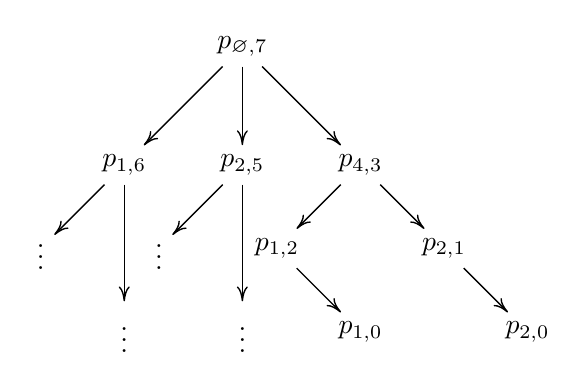
\begin{tikzpicture}[node distance=1.5cm]
      % níveis 0 e 1
      \node(p43)                    {$p_{4,3}$};
      \node(p25)  [left of=p43]     {$p_{2,5}$};
      \node(p16)  [left of=p25]     {$p_{1,6}$};
      \node(p07)  [above of=p25] {$p_{\varnothing,7}$};

      \seta(p07) -- (p16);
      \seta(p07) -- (p25);
      \seta(p07) -- (p43);

      % nível 2   -- criar relevo aqui
      \node(x1)  [below left of=p16]   {$\vdots$};
      \node(x2)  [below right of=x1]   {$\vdots$};
      \node(x3)  [right of=x1]         {$\vdots$};
      \node(x4)  [below right of=x3]   {$\vdots$};
      \node(p12) [below left of=p43]   {$p_{1,2}$};
      \node(p21) [below right of=p43]  {$p_{2,1}$};

      \seta(p16) -- (x1);
      \seta(p16) -- (x2);
      \seta(p25) -- (x3);
      \seta(p25) -- (x4);
      \seta(p43) -- (p12);
      \seta(p43) -- (p21);

      % nível 3
      \node(p10) [below right of=p12]  {$p_{1,0}$};
      \node(p20) [below right of=p21]  {$p_{2,0}$};

      \seta(p12) -- (p10);
      \seta(p21) -- (p20);
   \end{tikzpicture}
\end{minipage}
\hfill
\begin{minipage}{0.4\textwidth}
\end{minipage}
\end{figure}
\end{document}
